% Short-paper draft (RESEARCH_RECORD.md); no venue presumed.
% Build:  latexmk -pdf -outdir=build main.tex
\documentclass[11pt]{article}
\usepackage[a4paper,margin=25mm]{geometry}
\usepackage[T1]{fontenc}
\usepackage{lmodern}
\usepackage{microtype}
\usepackage{amsmath,amssymb,amsthm}
\usepackage{float}
\usepackage{graphicx}
\usepackage{booktabs}
\usepackage{xcolor}
\usepackage[numbers,square,sort&compress]{natbib}
\usepackage[hidelinks]{hyperref}
\usepackage[capitalise,nameinlink]{cleveref}

\newtheorem{theorem}{Theorem}[section]
\newtheorem{proposition}[theorem]{Proposition}
\newtheorem{lemma}[theorem]{Lemma}
\newtheorem{corollary}[theorem]{Corollary}
\theoremstyle{remark}
\newtheorem{remark}[theorem]{Remark}

% Notation and helpers for the manuscript.

% Placeholder for text that waits on a later week of FINAL_RESEARCH_PLAN.md.
\newcommand{\pending}[1]{\par\noindent\fbox{\parbox{0.97\linewidth}{\color{red!70!black}\small\textbf{Pending:} #1}}\par}
% Marker for a reference or statement that still has to be verified.
\newcommand{\verify}[1]{{\color{red!70!black}[verify: #1]}}

% Vectors and matrices
\newcommand{\vu}{\boldsymbol{u}}
\newcommand{\vv}{\boldsymbol{v}}
\newcommand{\vf}{\boldsymbol{f}}
\newcommand{\vc}{\boldsymbol{c}}
\newcommand{\vd}{\boldsymbol{d}}
\newcommand{\vg}{\boldsymbol{g}}
\newcommand{\ve}{\boldsymbol{e}}
\newcommand{\vp}{\boldsymbol{p}}
\newcommand{\vr}{\boldsymbol{r}}
\newcommand{\vw}{\boldsymbol{w}}
\newcommand{\vlam}{\boldsymbol{\lambda}}
\newcommand{\vell}{\boldsymbol{\ell}}
\newcommand{\vmu}{\boldsymbol{\mu}}
\newcommand{\mK}{\boldsymbol{K}}
\newcommand{\mB}{\boldsymbol{B}}
\newcommand{\mX}{\boldsymbol{X}}
\newcommand{\mV}{\boldsymbol{V}}
\newcommand{\mW}{\boldsymbol{W}}
\newcommand{\mI}{\boldsymbol{I}}
\newcommand{\Bp}{\mB^{+}}

% Approximations
\newcommand{\ut}{\tilde{\vu}}
\newcommand{\lt}{\tilde{\vlam}}
\newcommand{\gt}{\tilde{\vg}}
\newcommand{\et}{\tilde{\ve}}
\newcommand{\uh}{\hat{\vu}}
\newcommand{\gh}{\hat{\vg}}
\newcommand{\lh}{\hat{\vlam}}

% Sets
\newcommand{\Aplus}{\mathcal{A}_{+}}
\newcommand{\Acon}{\mathcal{A}}
\newcommand{\Ahat}{\hat{\mathcal{A}}}
\newcommand{\Miss}{\mathcal{M}}

% Operators and norms
\newcommand{\T}{^{\mathsf{T}}}
\newcommand{\norm}[1]{\lVert #1 \rVert}
\newcommand{\normK}[1]{\lVert #1 \rVert_{\mK}}
\newcommand{\normKi}[1]{\lVert #1 \rVert_{\mK^{-1}}}
\newcommand{\normXi}[1]{\lVert #1 \rVert_{\mX^{-1}}}
\newcommand{\pos}[1]{(#1)^{+}}
\newcommand{\rhob}{\bar{\rho}}
\newcommand{\Dstar}{\Delta^{\star}}
\newcommand{\lmr}{\vell^{\star}}


\title{Efficiency and limitations of optimised-multiplier error certificates for discrete contact problems}
\author{Author list to be supplied}
\date{}

\begin{document}
\maketitle

\begin{abstract}
Reliable error bounds are essential for assessing approximate solutions of unilateral contact problems, particularly those obtained from reduced-order models. For discrete frictionless contact problems, an established feasible-pair certificate bounds the energy-norm error using an equilibrium residual, a complementarity term, and an arbitrary nonnegative multiplier. However, its efficiency under convex-surrogate multiplier optimisation remains insufficiently characterised. This study derives an efficiency bound relating the optimised certificate to the true displacement error and the complementarity between exact contact forces and approximate gaps. For the stiffness-based inner product, the surrogate-minimising multiplier is shown to solve a contact problem with a shifted obstacle. It coincides with the exact multiplier if and only if the approximate gap lies between zero and twice the exact gap, in which case the certificate equals the true error. An explicit counterexample establishes worst-case square-root degradation within this certificate family, even under unrestricted multiplier optimisation. Furthermore, omitting a strictly active constraint from the multiplier support produces a positive asymptotic certificate floor for a fixed problem. Numerical experiments on two finite element benchmarks and 3000 random constrained quadratic problems found no violation of the tested properties. In the controlled support-restriction experiments, restricted certificates exceed unrestricted certificates by factors greater than $5\times10^4$. These findings indicate the importance of active-set consistency and multiplier support for certificate sharpness. Since the exactness condition depends on the unknown full-order solution, and the numerical evidence is small in scale, computable criteria for assessing certificate efficiency remain an important direction for future work.
\end{abstract}

\noindent\textbf{Keywords:} a posteriori error estimation; frictionless contact; variational inequalities; error certificate; effectivity; complementarity; reduced-order models.

% Section 1: introduction (short-paper outline, RESEARCH_RECORD.md). Statements about the literature mean
% "not found in the texts read"; gate S1 was closed with a stated risk (two sources unread), see Sec. 7.

\section{Introduction}\label{sec:intro}

A posteriori error estimation plays an important role in assessing the reliability of numerical approximations to contact and obstacle problems.
In unilateral contact mechanics, an approximate displacement must satisfy non-penetration constraints, while the associated contact forces must
remain nonnegative and obey complementarity conditions. These inequalities distinguish contact problems from unconstrained elliptic equations and
introduce additional difficulties in error estimation. Established error certificates address these difficulties by combining an equilibrium
residual with a complementarity contribution involving a feasible displacement approximation and a nonnegative multiplier. Such estimates have
been developed in the functional framework for obstacle problems \cite{repin2000,repin2007}, through finite element error estimators
\cite{veeser2001,braess2005,krause2015}, and for discrete variational inequalities and reduced-order contact models
\cite{zhang2016cr,zhang2016thesis}. Since the multiplier used in the certificate need not coincide with that of the numerical approximation, it
can be selected to improve the resulting bound. One established strategy is to minimise a convex quadratic surrogate of the certificate, leading
to a linear complementarity problem \cite{repin2007,zhang2016thesis}. We refer to this strategy as S1.

The reliability and efficiency of a posteriori error estimators for obstacle and Signorini problems have been investigated extensively. Existing
finite element analyses establish efficiency estimates involving primal and multiplier errors and identify the influence of contact regions on
estimator behaviour \cite{veeser2001,braess2005,krause2015}. Reduced-basis methods for variational inequalities have also revealed a possible
square-root difference between error bounds \cite{haasdonk2012}. A duality approach with strictly feasible approximations reports bounds that numerically follow the convergence rate of the reduced-basis error in two model problems, without deriving an efficiency bound \cite{zhang2014arxiv}. More generally, primal--dual gap formulations and error identities provide rigorous
relationships among equilibrium residuals, approximation errors and contact-complementarity terms \cite{bartels2025,repin2018}. These results
establish the mathematical foundations of contact-aware error estimation. They also show that the interaction between displacement accuracy and
contact consistency is an important consideration when interpreting an error bound.

Despite these developments, the efficiency of the particular feasible-pair certificate obtained through convex-surrogate multiplier optimisation
remains less explicitly characterised. To the best of our knowledge, the literature does not provide an explicit characterisation of when the
optimised certificate coincides with the true displacement error. Furthermore, it neither demonstrates that convergence-rate degradation may
persist under unrestricted multiplier optimisation nor analyses the asymptotic certificate floor caused by omitted strictly active contact-force
components. While established primal--dual energy identities provide closely related estimates, they leave open key questions regarding the
surrogate-minimising multiplier.

To address this gap, the present study investigates the relationship between the optimised certificate, the true displacement error and the
complementarity between exact contact forces and approximate contact gaps. We first establish an efficiency estimate that quantifies this relationship
for a general symmetric positive-definite inner product. For the stiffness-based inner product, we interpret the surrogate-minimising multiplier as
the contact-force solution of a problem with a shifted obstacle. This interpretation enables a precise characterisation of the conditions under
which the optimised multiplier recovers the exact multiplier and the resulting certificate equals the true energy error. We then examine the
limitations of multiplier optimisation through an explicit counterexample demonstrating unavoidable worst-case square-root degradation within the
considered certificate family. A separate analysis shows that restricting the multiplier support so that a strictly active contact constraint is
omitted can produce a positive asymptotic certificate floor. These findings are complemented by bounds that quantify the contribution of missed
contact constraints to certificate efficiency.

The theoretical results are examined numerically using two finite element contact benchmarks, controlled approximation sequences and randomly
generated constrained quadratic problems. We also consider elementary feasibility and snap-to-contact corrections of reduced-order predictions to
illustrate the relationship between active-set consistency, certificate efficiency and displacement accuracy. The investigation is analytical in
scope: it does not propose a new error certificate, multiplier-selection algorithm or reduced-order method. Moreover, the conditions for exact
certification involve quantities from the unknown full-order solution and are therefore intended to explain certificate behaviour rather than
provide a directly applicable online exactness test. The numerical experiments are designed to verify the derived properties rather than demonstrate
computational acceleration.

The remainder of the paper is organised as follows. Section~\ref{sec:setting} presents the mathematical formulation and feasible-pair error
certificate. Section~\ref{sec:analysis} investigates certificate efficiency and conditions for exact certification. Section~\ref{sec:failure}
examines square-root convergence degradation, missed contact constraints and the effects of restricted multiplier support.
Section~\ref{sec:results} provides numerical verification of the theoretical results, while Section~\ref{sec:application} illustrates their
application to corrections of reduced-order contact predictions. Section~\ref{sec:conclusions} summarises the principal findings, limitations
and directions for future research. Appendix~\ref{app:e3} presents the random-instance verification results and supplementary numerical diagnostics.

% Section 2: setting and the feasible-pair certificate (known results, cited).

\section{Setting and the feasible-pair certificate}\label{sec:setting}

\subsection{Full-order contact problem}
The discrete frictionless unilateral contact problem is considered:
\begin{equation}\label{eq:fom}
  \mK\vu-\mB\T\vlam=\vf,\qquad \vg:=\mB\vu-\vc\ge\boldsymbol 0,\qquad \vlam\ge\boldsymbol 0,\qquad \vlam\T\vg=0,
\end{equation}
Here, $\vu\in\mathbb R^{N}$ denotes the displacement and $\vlam\in\mathbb R^{n_c}$ the contact forces. The matrix $\mK$ is assumed symmetric
positive definite and $\mB\in\mathbb R^{n_c\times N}$ has full row rank. Positive definiteness gives a strictly convex energy and hence a unique
displacement $\vu$; full row rank makes the constraints feasible for every $\vc$ (so $\vu$ exists) and $\mB\T$ injective, which gives a unique multiplier
$\vlam=(\mB\mB\T)^{-1}\mB(\mK\vu-\vf)$. These assumptions therefore ensure existence and uniqueness of the primal--dual solution $(\vu,\vlam)$. The problem data may depend on a parameter
$\vmu$, which is suppressed when fixed. The strictly active set $\Aplus$ and the contact set $\Acon$ are defined by
\begin{equation}\label{eq:sets}
  \Aplus:=\{i:\lambda_i>0\}\subseteq\Acon:=\{i:g_i=0\}
\end{equation}
for the full-order solution.

A Galerkin reduced-order model \cite{balajewicz2016} approximates $\vu\approx\ut=\mV\vu_r$ and
$\vlam\approx\lt=\mW\vlam_r$ using primal and dual bases and solves the projected complementarity problem. The reconstructed pair satisfies
the reduced conditions but may violate full-order feasibility.
Section~\ref{sec:application} constructs a feasible displacement $\uh$, with $\gh:=\mB\uh-\vc\ge\boldsymbol 0$. The analysis in
Sections~\ref{sec:setting}--\ref{sec:failure} applies to any feasible approximation, with error $\ve:=\vu-\uh$. Errors and certificates are
measured relative to the full-order finite element solution, excluding the discretisation error of the continuous problem; the latter is addressed by finite element a posteriori estimators
\cite{veeser2001,braess2005,weiss2010,krause2015}.

\subsection{Inner product and coercivity constants}
Let $\mX$ be symmetric positive definite and let $0<\alpha_X\le\gamma_X$ satisfy
\begin{equation}\label{eq:equiv}
  \alpha_X\,\vv\T\mX\vv\le\vv\T\mK\vv\le\gamma_X\,\vv\T\mX\vv\qquad\text{for all }\vv\in\mathbb R^N,
\end{equation}
and define $s:=(\gamma_X/\alpha_X)^{1/2}\ge1$. For constant stiffness, choosing $\mX=\mK$ gives $\alpha_X=\gamma_X=s=1$.

For an affine stiffness $\mK(\vmu)=\sum_q\theta_q(\vmu)\mK_q$, with $\theta_q\ge0$ and $\mK_q$ symmetric positive semidefinite, the reference
matrix is chosen as $\mX=\mK(\bar\vmu)$. If $\theta_q(\bar\vmu)>0$ and $\theta_q(\vmu)>0$ for every nonzero $\mK_q$, the minimum and maximum coefficient ratios
provide positive spectral-equivalence constants without eigenvalue computations. Vanishing coefficients require a separate positive coercivity
bound. When all coefficients are positive, \eqref{eq:equiv} holds with
$\alpha_X=\min_q\theta_q(\vmu)/\theta_q(\bar\vmu)$ and $\gamma_X=\max_q\theta_q(\vmu)/\theta_q(\bar\vmu)$.

The Euclidean choice $\mX=\mI$ serves as a baseline. The extreme eigenvalues of $\mK$ give $s=\kappa(\mK)^{1/2}$; conservative eigenvalue
bounds generally yield a larger value.

\subsection{The feasible-pair certificate}
For a multiplier candidate $\vell\ge\boldsymbol 0$ define
\begin{equation}\label{eq:certificate}
  \rhob(\vell):=\frac{\normXi{\vf+\mB\T\vell-\mK\uh}}{\sqrt{\alpha_X}},\qquad
  \eta(\vell):=\vell\T\gh,\qquad
  \Dstar(\vell):=\tfrac12\Big(\rhob(\vell)+\sqrt{\rhob(\vell)^2+4\eta(\vell)}\Big).
\end{equation}

The following established result provides an upper bound on the energy-norm error for any feasible displacement approximation
\cite[Prop.~4.3]{zhang2016cr}, \cite[Prop.~3.3.6]{zhang2016thesis}.

\begin{proposition}[feasible-pair error bound]\label{prop:certificate}
Let $\uh$ be a feasible displacement approximation, $\gh\ge\boldsymbol 0$. Then, for every nonnegative multiplier $\vell\ge\boldsymbol 0$, $\normK{\ve}\le\Dstar(\vell)$.
\end{proposition}
Related functional bounds for obstacle problems involve arbitrary nonnegative multipliers, equilibrium residuals, and complementarity terms
\cite[(2.12)--(2.13)]{repin2007}. Finite element counterparts appear in \cite[Lemma~1]{braess2005} and \cite[Sec.~4.2]{krause2015}.
\begin{proof}
By \eqref{eq:fom}, $\mK\ve=\vr+\mB\T(\vlam-\vell)$ with $\vr:=\vf+\mB\T\vell-\mK\uh$, and $\mB\ve=\vg-\gh$. Hence
$\normK{\ve}^2=\ve\T\vr+(\vg-\gh)\T(\vlam-\vell)$. The second term equals
$\vg\T\vlam-\vg\T\vell-\gh\T\vlam+\gh\T\vell\le\eta(\vell)$, since $\vg\T\vlam=0$ and all other products of non-negative vectors
are non-negative. With $\ve\T\vr\le\normK{\ve}\normKi{\vr}\le\normK{\ve}\rhob(\vell)$ by \eqref{eq:equiv}, $\normK{\ve}$ satisfies
$\normK{\ve}^2-\rhob\normK{\ve}-\eta\le0$, whose positive root is $\Dstar(\vell)$.
\end{proof}

\subsection{Minimum-residual multiplier}
Following the established surrogate-minimisation approach \cite{zhang2016thesis}, the nonnegative multiplier is selected by solving
\begin{equation}\label{eq:phi}
  \Phi(\vell):=\rhob(\vell)^2+\eta(\vell),\qquad \lmr:=\operatorname*{arg\,min}_{\vell\ge\boldsymbol 0}\Phi(\vell).
\end{equation}
Since $\mB$ has full row rank, the Hessian $2\mB\mX^{-1}\mB\T/\alpha_X$ is positive definite. Hence $\Phi$ is strictly convex and has a unique
minimiser $\lmr$, characterised by a linear complementarity problem with $n_c$ unknowns. Related functional-majorant minimisations for continuous
obstacle problems are established in \cite{repin2000,repin2007}.

\begin{lemma}[surrogate--certificate equivalence]\label{lem:phi}
For every nonnegative multiplier $\vell\ge\boldsymbol 0$, $\Phi(\vell)\le\Dstar(\vell)^2\le\frac43\Phi(\vell)$.
\end{lemma}
\begin{proof}
Let $\rho=\rhob(\vell)$, $\eta=\eta(\vell)$ and $P=\rho^2+\eta$. If $P=0$, then $\rho=\eta=0$, $\Dstar=0$, and both bounds hold trivially. Otherwise, ${\Dstar}^2=\rho\Dstar+\eta\ge P$, since $\Dstar\ge\rho$. For the upper bound, $\sqrt{\rho^2+4\eta}=\sqrt{4P-3\rho^2}$, so
\[
  \Dstar=\tfrac12\Big(\rho+\sqrt{4P-3\rho^2}\Big),
\]
which, as a function of $\rho\in[0,\sqrt P]$, attains its maximum $2\sqrt{P/3}$ at $\rho=\sqrt{P/3}$. Consequently, ${\Dstar}^2\le4P/3\le\frac43\Phi$.
\end{proof}

\subsection{Relation to the primal--dual gap}
Equation \eqref{eq:fom} represents the optimality conditions for minimising $J(\vv):=\frac12\vv\T\mK\vv-\vf\T\vv$ subject to $\mB\vv\ge\vc$, with
dual function $\mathcal D(\vell):=-\frac12(\vf+\mB\T\vell)\T\mK^{-1}(\vf+\mB\T\vell)+\vell\T\vc$ for $\vell\ge\boldsymbol 0$.

The primal--dual gap $J(\uh)-\mathcal D(\vell)$ provides an established basis for error estimation \cite{zhangs2020}. For $\mX=\mK$, it involves the same residual and complementarity terms
as the feasible-pair certificate. The identities in Proposition~\ref{prop:gap} are closely related to established primal--dual gap and energy identities \cite{bartels2025}. They also show that, for the same
multiplier, the certificate does not exceed the corresponding gap-based error bound.

\begin{proposition}\label{prop:gap}
Let $\uh$ be feasible, $\vell\ge\boldsymbol 0$, $\mX=\mK$, and $G(\uh,\vell):=J(\uh)-\mathcal D(\vell)$. Then
\begin{equation}\label{eq:gap}
  G(\uh,\vell)=\tfrac12\rhob(\vell)^2+\eta(\vell),\qquad
  J(\uh)-J(\vu)=\tfrac12\normK{\ve}^2+\vlam\T\gh,\qquad
  \normK{\ve}\le\Dstar(\vell)\le\sqrt{2G(\uh,\vell)},
\end{equation}
with equality in the last inequality if and only if $\eta(\vell)=0$.
\end{proposition}
\begin{proof}
With $\vw:=\vf+\mB\T\vell$, $J(\uh)-\mathcal D(\vell)=\frac12\uh\T\mK\uh-\vw\T\uh+\frac12\vw\T\mK^{-1}\vw+\vell\T(\mB\uh-\vc)=\frac12\normKi{\mK\uh-\vw}^2+\vell\T\gh$.
Next, $J(\uh)-J(\vu)=\frac12\normK{\ve}^2+(\mK\vu-\vf)\T(\uh-\vu)$ and $\mK\vu-\vf=\mB\T\vlam$, $\mB(\uh-\vu)=\gh-\vg$, $\vlam\T\vg=0$. Finally,
${\Dstar}^2=\rhob\Dstar+\eta\le\frac12(\rhob^2+{\Dstar}^2)+\eta$ gives ${\Dstar}^2\le\rhob^2+2\eta=2G$, with equality if and only if $\rhob=\Dstar$, i.e.
$\eta=0$; the first inequality is Proposition~\ref{prop:certificate}.
\end{proof}

The second identity in \eqref{eq:gap} identifies $\vlam\T\gh$ as the contribution to the primal energy difference beyond one-half of the squared
energy error. Its continuous counterpart appears in \cite{bartels2025}. For $\mX=\mK$, the lower bounds on the certificate also apply to the
corresponding gap-based error bound, since $\sqrt{2G}\ge\Dstar$. For general $\mX$, the residual norms differ, and this transfer need not hold.
% Sections 3 (efficiency) and 4 (failure mechanisms).
% Source: THEOREM_certificate_efficiency.md and ANALYSIS_T1_T3.md (project root).

\section{Efficiency of the certificate}\label{sec:analysis}

Proposition~\ref{prop:certificate} establishes the reliability of the feasible-pair certificate. This section examines its efficiency for the optimised
multiplier, in terms of the true displacement error, identifies conditions for bounded effectivity, and characterises exact certification. The results
apply to any feasible displacement approximation.

\subsection{An efficiency bound in the true error}

The key quantity is the complementarity of the \emph{exact} multiplier with the \emph{approximate} gap,
$\vlam\T\gh$. Since $\vlam\T\vg=0$ and $\gh=\vg-\mB\ve$,
\begin{equation}\label{eq:excess-identity}
  0\le\vlam\T\gh=-\vlam\T\mB\ve=-\sum_{i\in\Aplus}\lambda_i(\mB\ve)_i .
\end{equation}
For a row set $\Miss$, let $\vlam_{\Miss}$ denote $\vlam$ with entries outside $\Miss$ set to zero, and define
\begin{equation}\label{eq:intensity}
  m(\Miss):=\normKi{\mB\T\vlam_{\Miss}} .
\end{equation}
$m(\Aplus)=\normKi{\mB\T\vlam}=\normK{\vu-\mK^{-1}\vf}$ is the energy distance between the constrained and the unconstrained
solution, a measure of the contact intensity.

\begin{theorem}[efficiency]\label{thm:efficiency}
For every feasible $\uh$,
\begin{equation}\label{eq:efficiency}
  \normK{\ve}\ \le\ \Dstar(\lmr)\ \le\ \frac{2}{\sqrt3}\,\Phi(\lmr)^{1/2}\ \le\ \frac{2}{\sqrt3}\Big(s^2\normK{\ve}^2+\vlam\T\gh\Big)^{1/2},
\end{equation}
and $\vlam\T\gh\le m(\Aplus)\,\normK{\ve}$.
\end{theorem}
\begin{proof}
The first inequality is Proposition~\ref{prop:certificate} and the second is Lemma~\ref{lem:phi}. For the third, the exact multiplier
$\vlam\ge\boldsymbol 0$ is admissible in \eqref{eq:phi}, so $\Phi(\lmr)\le\Phi(\vlam)$. At $\vell=\vlam$ the residual is
$\vf+\mB\T\vlam-\mK\uh=\mK\ve$, and $\mK\preceq\gamma_X\mX$ is equivalent to $\mK\mX^{-1}\mK\preceq\gamma_X\mK$; hence
$\rhob(\vlam)^2=\ve\T\mK\mX^{-1}\mK\ve/\alpha_X\le s^2\normK{\ve}^2$, while $\eta(\vlam)=\vlam\T\gh$. The last claim follows from
\eqref{eq:excess-identity} and the Cauchy--Schwarz inequality in the $\mK^{-1}$/$\mK$ pairing.
\end{proof}

The first two inequalities in \eqref{eq:efficiency} are established results. For $\mX=\mK$, the identity
$\Phi(\vlam)=\normK{\ve}^2+\vlam\T\gh$ follows from the primal energy relation in Proposition~\ref{prop:gap}; its continuous counterpart
appears in \cite{bartels2025}. Theorem~\ref{thm:efficiency} extends this comparison to the computable surrogate-minimising multiplier,
introducing only the factor $2/\sqrt3$ and requiring no separate multiplier-error term.

Related studies establish efficiency estimates involving primal and multiplier errors \cite{veeser2001,braess2005,krause2015}, identify
contact-related contributions near free boundaries \cite{krause2015,weiss2010,braess2005}, and examine square-root differences between residual
bounds for reduced-basis approximations \cite{haasdonk2012}. Functional majorants for obstacle problems have also been minimised over
nonnegative multipliers \cite{repin2000,repin2007}, while primal--dual error identities identify contributions associated with contact-set mismatch
\cite{repin2018,bartels2025}. The present analysis focuses on the efficiency of the finite-dimensional surrogate-minimising certificate relative to
the primal error. Equivalent explicit statements of the efficiency bound, active-set consistency result, sharp half-rate example, and force-weighted
missed-row bound were not identified in the examined literature
\cite{haasdonk2012,zhang2016cr,zhang2016thesis,zhangs2020,bartels2025,ashby2024,veeser2001,braess2005,weiss2010,krause2015,nochetto2003,burkovska2015,benaceur2020,repin2000,repin2007,repin2018}.
This assessment is limited to the source versions examined, including preprints where published versions were unavailable.

\begin{remark}[inexact minimisation; sharper special case]\label{rem:inexact}
Any computed nonnegative multiplier $\tilde\vell$ remains admissible for certification. If
$\Phi(\tilde\vell)\le\Phi(\lmr)+\delta$, then
$\Dstar(\tilde\vell)\le\frac{2}{\sqrt3}(s^2\normK{\ve}^2+\vlam\T\gh+\delta)^{1/2}$.
If $\eta(\lmr)=0$, then $\Dstar(\lmr)=\rhob(\lmr)=\Phi(\lmr)^{1/2}$, and the factor $2/\sqrt3$ is unnecessary.
\end{remark}

\begin{corollary}[effectivity]\label{cor:effectivity}
Let $\mathrm{eff}:=\Dstar(\lmr)/\normK{\ve}$ for $\ve\ne\boldsymbol 0$.
\begin{enumerate}
\item[(a)] In general, $1\le\mathrm{eff}\le\frac{2}{\sqrt3}\big(s^2+m(\Aplus)/\normK{\ve}\big)^{1/2}$. Along a sequence with bounded $s$ and $m(\Aplus)$,
the certificate is therefore at worst of order $\normK{\ve}^{1/2}$; this upper rate need not be attained, but it is sharp in the
worst case (Proposition~\ref{prop:half-rate}).
\item[(b)] \emph{Active-set consistency.} If $\hat g_i=0$ for every $i\in\Aplus$, then $\vlam\T\gh=0$ and
\begin{equation}\label{eq:eff-consistent}
  1\le\mathrm{eff}\le\frac{2}{\sqrt3}\,s ;
\end{equation}
in particular $\mathrm{eff}\le2/\sqrt3\approx1.155$ for $\mX=\mK$, and $\mathrm{eff}\le\frac{2}{\sqrt3}\kappa(\mK)^{1/2}$ for $\mX=\mI$.
\item[(c)] If $\vlam\T\gh\le C\normK{\ve}^2$, then $\mathrm{eff}\le\frac{2}{\sqrt3}(s^2+C)^{1/2}$.
\end{enumerate}
\end{corollary}

Part (b) guarantees bounded effectivity when the approximation is in contact on every strictly active row. Uniformity across a family of problems
also requires bounded $s$. For $\mX=\mK(\vmu)$, $s=1$. With a positive affine stiffness decomposition and $\mX=\mK(\bar\vmu)$, the
coefficient ratios provide parameter-dependent bounds. For $\mX=\mI$, $s=\kappa(\mK)^{1/2}$ when exact extreme eigenvalues are used; this
factor may deteriorate under mesh refinement.

\begin{remark}[comparison with the primal--dual gap]\label{rem:gap-comparison}
Let $\mX=\mK$. The dual function $\mathcal D$ is strictly concave and maximised at $\vlam$, so
$\operatorname{arg\,min}_{\vell\ge0}G(\uh,\vell)=\vlam$ and
$\min_{\vell\ge0}G(\uh,\vell)=\frac12\normK{\ve}^2+\vlam\T\gh$. Consequently,
\[
  \Dstar(\vlam)\le\sqrt{2G(\uh,\vlam)}
  =\big(\normK{\ve}^2+2\vlam\T\gh\big)^{1/2}.
\]
This bound uses the exact multiplier, whose computation requires solving the full-order dual problem. By contrast,
Theorem~\ref{thm:efficiency} concerns the surrogate minimiser $\lmr$, which generally differs from $\vlam$ and need not minimise $\Dstar$.
The squared upper bounds are $\frac43(\normK{\ve}^2+\vlam\T\gh)$ and
$\normK{\ve}^2+2\vlam\T\gh$, respectively; the former is smaller when
$\vlam\T\gh>\frac12\normK{\ve}^2$. Thus, the efficiency result is a modest extension of the established gap identity, whereas the exactness and
failure-mechanism results require separate analysis.
\end{remark}

\subsection{S1 as a contact problem; exact certification}\label{sec:s1-contact}

For $\mX=\mK$ ($\alpha_X=1$), the surrogate-minimising multiplier solves a shifted contact problem. Define
$\vu_f:=\mK^{-1}\vf$ and $\mathbf H:=\mB\mK^{-1}\mB\T$, which is symmetric positive definite.

\begin{proposition}[S1 is a shifted contact problem]\label{prop:shifted}
Let $\mX=\mK$ and let $\uh$ be feasible. Then $\lmr$ solves
\begin{equation}\label{eq:shifted-lcp}
  \vell\ge\boldsymbol 0,\qquad \mathbf H\vell+\mB\vu_f-\vc'\ge\boldsymbol 0,\qquad \vell\T\big(\mathbf H\vell+\mB\vu_f-\vc'\big)=0,\qquad
  \vc':=\vc+\tfrac12\gh ,
\end{equation}
that is, $(\vu',\lmr)$ with $\vu':=\mK^{-1}(\vf+\mB\T\lmr)$ is the solution of the contact problem \eqref{eq:fom} with obstacle $\vc'$.
Moreover $\rhob(\lmr)=\normK{\uh-\vu'}$, the displacement $\uh$ is feasible for the problem with obstacle $\vc'$, and $\vu'$ is feasible for the
original problem.
\end{proposition}
\begin{proof}
$\nabla\Phi(\vell)=2\mB\mK^{-1}(\vf+\mB\T\vell-\mK\uh)+\gh=2(\mathbf H\vell+\mB\vu_f-\mB\uh)+\gh=2(\mathbf H\vell+\mB\vu_f-\vc-\tfrac12\gh)$, because $\mB\uh=\vc+\gh$.
$\Phi$ is strictly convex, so $\lmr$ is characterised by $\vell\ge\boldsymbol 0$, $\nabla\Phi\ge\boldsymbol 0$, $\vell\T\nabla\Phi=0$, which are \eqref{eq:shifted-lcp}; these are the
optimality conditions of \eqref{eq:fom} with obstacle $\vc'$, whose solution is unique. Then $\vf+\mB\T\lmr-\mK\uh=\mK(\vu'-\uh)$ gives
$\rhob(\lmr)=\normK{\uh-\vu'}$. Finally $\mB\uh=\vc+\gh\ge\vc'$ and $\mB\vu'\ge\vc'\ge\vc$.
\end{proof}

\begin{corollary}[exact certification]\label{cor:exact}
Let $\mX=\mK$ and $\boldsymbol 0\le\gh\le2\vg$ componentwise (in particular, $\hat g_i=0$ wherever $g_i=0$, so $\uh$ is in contact on the whole
contact set, and open rows are at most twice as open as in the exact solution). Then $\lmr=\vlam$, $\vu'=\vu$, and
\begin{equation}\label{eq:exact}
  \Dstar(\lmr)=\normK{\ve}.
\end{equation}
Conversely, for $\mX=\mK$ and feasible $\uh$, $\lmr=\vlam$ implies $\boldsymbol 0\le\gh\le2\vg$. Hence $\lmr=\vlam$ if and only if $\boldsymbol 0\le\gh\le2\vg$.
\end{corollary}
\begin{proof}
$(\vu,\vlam)$ satisfies \eqref{eq:shifted-lcp}: $\mB\vu-\vc'=\vg-\tfrac12\gh\ge\boldsymbol 0$, and $\lambda_i>0$ implies $g_i=0$, hence $\hat g_i=0$ and
$(\vg-\frac12\gh)_i=0$. By uniqueness, $\lmr=\vlam$ and $\vu'=\vu$. Then $\rhob(\lmr)=\normK{\uh-\vu}=\normK{\ve}$ and $\vlam\T\gh=0$.
Conversely, if $\lmr=\vlam$, then $\vu'=\mK^{-1}(\vf+\mB\T\vlam)=\vu$, and \eqref{eq:shifted-lcp} gives $\vg-\frac12\gh=\mB\vu-\vc'\ge\boldsymbol 0$, that is $\gh\le2\vg$; together with $\gh\ge\boldsymbol 0$ this is the condition.
(The converse implication from exact certificate effectivity to exact multiplier recovery is not asserted.)
\end{proof}

Corollary~\ref{cor:exact} strengthens the bounded-effectivity result for $\mX=\mK$ to exact certification. Because the condition involves the
unknown exact gap, it provides an analytical characterisation rather than an online test. Thus, reliability holds for any feasible approximation,
active-set consistency ensures bounded effectivity, and the stronger gap condition yields exact certification.

The shifted-contact interpretation also applies to a multiplier restricted to a support $S$. The corresponding displacement $\vu'_S$ satisfies only
the shifted constraints indexed by $S$ and may violate omitted constraints. Nevertheless, the certificate remains valid because $\uh$ is feasible
and $\lmr_S\ge0$, with residual $\rhob(\lmr_S)=\normK{\uh-\vu'_S}$. If $S$ omits a strictly active row, then $\vu'_S\ne\vu$; otherwise,
equilibrium and the injectivity of $\mB\T$ would imply $\lambda_i=0$ outside $S$, contradicting strict activity. This explains the restricted-support
certificate floor established below.

\section{Failure mechanisms}\label{sec:failure}

This section examines two limitations of certificate efficiency. The first arises when contact constraints that are strictly active in the exact
solution remain open in the approximation. The second results from excluding strictly active constraints from the multiplier support.

\subsection{The half rate cannot be removed by the multiplier}

\begin{proposition}[square-root degradation of the certificate family]\label{prop:half-rate}
Without active-set consistency, no multiplier restores the full rate in the worst case within the certificate \eqref{eq:certificate}; this is a property of this family, not a bound for every error estimator. Let $N=2$, $n_c=1$, $\mK=\mI$,
$\mB=[1\ \,0]$, $\vc=0$, $\vf=(-1,0)\T$ and $\mX=\mK$. The solution is $\vu=\boldsymbol 0$, $\lambda=1$, and the feasible approximation
$\uh=(\varepsilon,0)\T$, $\varepsilon>0$, has $\normK{\ve}=\varepsilon$. Then
\begin{equation}\label{eq:half-rate}
  \min_{\ell\ge0}\Dstar(\ell)=\sqrt{\varepsilon(1+\varepsilon)}\quad(\text{attained at }\ell=1+\varepsilon),\qquad
  \min_{\ell\ge0}\frac{\Dstar(\ell)}{\normK{\ve}}=\Big(\frac{1+\varepsilon}{\varepsilon}\Big)^{1/2}\to\infty .
\end{equation}
\end{proposition}
\begin{proof}
Here $\hat g=\varepsilon$, $\rhob(\ell)=|\ell-1-\varepsilon|$ and $\eta(\ell)=\ell\varepsilon$; write $\Delta=\Dstar(\ell)$, which satisfies $\Delta^2=\rhob\Delta+\ell\varepsilon$. At
$\ell=1+\varepsilon$, $\rhob=0$ and $\Delta=\sqrt{\varepsilon(1+\varepsilon)}$. If $\ell\ge1+\varepsilon$, then $\Delta^2\ge\ell\varepsilon\ge\varepsilon(1+\varepsilon)$. If $\ell<1+\varepsilon$, then
$\Delta^2=(1+\varepsilon)\Delta-\ell(\Delta-\varepsilon)$. For $\Delta\ge\varepsilon$ this gives $\Delta^2\ge(1+\varepsilon)\Delta-(1+\varepsilon)(\Delta-\varepsilon)=\varepsilon(1+\varepsilon)$; for $\Delta<\varepsilon$ it gives
$\Delta^2\ge(1+\varepsilon)\Delta$, i.e.\ $\Delta\ge1+\varepsilon>\varepsilon$, a contradiction.
\end{proof}

The square-root gap between residual bounds for variational inequalities was observed in \cite[Remark~4.5]{haasdonk2012}. This example
demonstrates that the degradation persists under unrestricted multiplier optimisation within the considered certificate family. It arises because
the approximation leaves open a contact constraint that is strictly active in the exact solution; it does not establish a limitation for other error
estimators.

\begin{figure}[t]
\centering
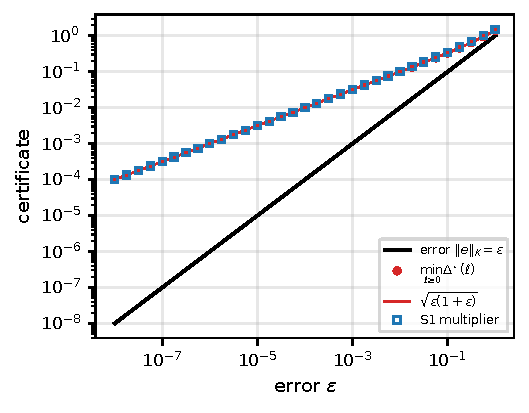
\includegraphics[width=0.62\linewidth]{figures/fig_halfrate}
\caption{The example of Proposition~\ref{prop:half-rate}. The error is $\varepsilon$ (slope $1$); the minimum of the certificate over all nonnegative multipliers,
computed numerically with the certificate code and compared with $\sqrt{\varepsilon(1+\varepsilon)}$, has slope $1/2$. The S1 multiplier, which in this example is
$\ell=1+\varepsilon/2$ and not the minimiser, gives a certificate that is visually indistinguishable from the minimum.}
\label{fig:half-rate}
\end{figure}

\subsection{Missed rows}

Corollary~\ref{cor:effectivity} covers the two extremes. For approximations that do not satisfy active-set consistency, the relevant complementarity contribution arises exclusively from strictly active
contact constraints that remain open in $\uh$.

\begin{theorem}[missed rows]\label{thm:missed}
Let $\Miss(\uh):=\{i\in\Aplus:\hat g_i>0\}$ be the rows of $\uh$ that are open although they carry a positive contact force in the
exact solution. Then
\begin{equation}\label{eq:missed}
  \vlam\T\gh=\sum_{i\in\Miss}\lambda_i\hat g_i=-\vlam_{\Miss}\T\mB\ve\le m(\Miss)\,\normK{\ve},
\end{equation}
and consequently
\begin{equation}\label{eq:missed-eff}
  \mathrm{eff}\le\frac{2}{\sqrt3}\Big(s^2+\frac{m(\Miss)}{\normK{\ve}}\Big)^{1/2}\le\frac{2}{\sqrt3}\Big(s+\sqrt{m(\Miss)/\normK{\ve}}\Big).
\end{equation}
\end{theorem}
\begin{proof}
In \eqref{eq:excess-identity} only rows with $\lambda_i>0$ and $\hat g_i>0$ contribute; on $\Aplus$, $\hat g_i=-(\mB\ve)_i$. The
bound follows from the Cauchy--Schwarz inequality, \eqref{eq:missed-eff} from Theorem~\ref{thm:efficiency} and
$\sqrt{a+b}\le\sqrt a+\sqrt b$.
\end{proof}

For $\Miss=\emptyset$, Theorem~\ref{thm:missed} recovers the active-set consistency bound. The bounds involving $m(\Miss)$ and
$m(\Aplus)$ are independent, since $m(\Miss)\le m(\Aplus)$ need not hold. In Proposition~\ref{prop:half-rate},
$\Miss=\{1\}$ and $m(\Miss)=1$, giving an upper bound proportional to $(\varepsilon^2+\varepsilon)^{1/2}$, within the factor
$2/\sqrt3$ of the exact minimum.

The energy-norm form \eqref{eq:missed} ignores how many rows are missed and how large their forces are. A localized
form makes this explicit and gives intermediate rates.

\begin{corollary}[localized form]\label{cor:localized}
With the notation of Theorem~\ref{thm:missed} (a maximum or norm over the empty set $\Miss=\emptyset$ is zero, and then $\vlam\T\gh=0$),
\begin{equation}\label{eq:localized}
  \vlam\T\gh\le\min\Big\{\norm{\vlam_{\Miss}}_2\,\norm{\gh_{\Miss}}_2,\ \norm{\vlam_{\Miss}}_1\max_{i\in\Miss}\hat g_i\Big\}.
\end{equation}
If, along a sequence of approximations, $\norm{\vlam_{\Miss}}_1\le C_\lambda\normK{\ve}^{a}$ for some $a\in[0,1]$ and
$\max_{\Miss}\hat g_i\le C_g\normK{\ve}$, then
\begin{equation}\label{eq:intermediate-rate}
  \Dstar(\lmr)\le\frac{2}{\sqrt3}\Big(s\,\normK{\ve}+(C_\lambda C_g)^{1/2}\normK{\ve}^{(1+a)/2}\Big).
\end{equation}
\end{corollary}
\begin{proof}
Hölder's inequality on the finite sum $\sum_{i\in\Miss}\lambda_i\hat g_i$, with exponents $(2,2)$ and $(1,\infty)$, then Theorem~\ref{thm:efficiency}. (The two bounds are separate; neither implies the other.)
\end{proof}

The exponent $a$ represents the assumed decay of contact forces on missed constraints, giving an upper rate of order
$\normK{\ve}^{(1+a)/2}$ when the constants remain bounded. This rate is not asserted to be sharp for every $a$. The gap condition holds with
$C_g=\max_i H_{ii}^{1/2}$, where $\mathbf H=\mB\mK^{-1}\mB\T$. Thus, the substantive additional assumption concerns the decay of
$\norm{\vlam_{\Miss}}_1$.

\subsection{Restricting the support of the multiplier}

The minimum-residual problem \eqref{eq:phi} has $n_c$ unknowns. For a row set $S$ let
$\lmr_S:=\operatorname{arg\,min}\{\Phi(\vell):\vell\ge\boldsymbol 0,\ \ell_i=0\text{ for }i\notin S\}$, and let $\mB_S$ denote the rows of $\mB$ in $S$ and
$S^c$ the complement.

\begin{theorem}[restricted support]\label{thm:support}
For every feasible $\uh$ and every $S$,
\begin{align}
  \Dstar(\lmr_S)&\le\frac{2}{\sqrt3}\Big(s^2\big(\normK{\ve}+m(S^c)\big)^2+\vlam\T\gh\Big)^{1/2},\label{eq:support-upper}\\
  \Dstar(\lmr_S)&\ge\frac{\sigma_S-\sqrt{\gamma_X}\,\normK{\ve}}{\sqrt{\alpha_X}},\qquad
  \sigma_S:=\min_{\vv\in\mathbb R^{|S|}}\normXi{\mB\T\vlam_{S^c}-\mB_S\T\vv}.\label{eq:support-lower}
\end{align}
Moreover $\sigma_S>0$ if and only if $\Aplus\not\subseteq S$.
\end{theorem}
\begin{proof}
The vector $\vlam_S$ is admissible, so $\Phi(\lmr_S)\le\Phi(\vlam_S)$. Its residual is $\mK\ve-\mB\T\vlam_{S^c}$, and
$\normXi{\vv}\le\sqrt{\gamma_X}\normKi{\vv}$ gives $\rhob(\vlam_S)\le s(\normK{\ve}+m(S^c))$; moreover $\vlam_S\T\gh\le\vlam\T\gh$. Lemma~\ref{lem:phi} yields
\eqref{eq:support-upper}. For \eqref{eq:support-lower}, any admissible $\vell$ has residual $\mK\ve-\mB\T(\vlam-\vell)$, so
$\sqrt{\alpha_X}\Dstar(\vell)\ge\normXi{\mB\T(\vlam-\vell)}-\normXi{\mK\ve}$; the first norm is at least $\sigma_S$ (drop the sign constraint) and
the second at most $\sqrt{\gamma_X}\normK{\ve}$. Finally, $\mB\T$ has full column rank, so $\mB\T\vlam_{S^c}\in\operatorname{range}\mB_S\T$ only if
$\vlam_{S^c}=\boldsymbol 0$.
\end{proof}

The quantity $\sigma_S$ depends on the exact multiplier and therefore provides an analytical diagnostic rather than an online support test. If
$S\supseteq\Aplus$, the restricted certificate satisfies the same efficiency bound as the unrestricted certificate. For a fixed problem and
support that omits a strictly active row,
\[
  \liminf_{\normK{\ve}\to0}\Dstar(\lmr_S)\ge\frac{\sigma_S}{\sqrt{\alpha_X}}>0.
\]
For varying problems or supports, a positive asymptotic floor requires $\sigma_S/\sqrt{\alpha_X}$ to remain bounded away from zero. Thus, missed
contact constraints in the displacement approximation may cause square-root degradation, whereas omitted active components in the multiplier support
may prevent certificate convergence. The gap-based support $S_t:=\{i:\hat g_i\le t\}$ contains $\Aplus$ whenever
$\norm{\mB\ve}_\infty\le t$.

% Numerical results (experiments E1--E3). Tables and figures are generated from saved results by
% experiments/tables.py and experiments/figures.py; no number in a table or figure is typed by hand.
\section{Numerical results}\label{sec:results}

The experiments verify the theoretical results of Sections~\ref{sec:setting}--\ref{sec:failure}.
All certificates use the S1-optimised multiplier with $\mX=\mK$, so $\alpha_X=s=1$. Three experiments are considered: E1 evaluates certificate
effectivity on two finite element benchmarks, E2 examines the restricted-support certificate floor, and E3 tests the theoretical properties on
random constrained quadratic problems. Results are pooled over three random seeds, $0$, $1$, and $2$.

\subsection{Benchmarks and corrections}\label{sec:setup}
\begin{table}[t]
\centering\small
\caption{The finite element benchmarks (read from the benchmark definitions and the settings of the code base).}
\label{tab:benchmarks}
% generated by experiments/tables.py; seeds [0, 1, 2]
\begin{tabular}{lll}
\hline
 & membrane & block \\
\hline
element & Quad4, scalar Laplace (2D) & Hex8, linear elasticity (3D) \\
mesh & $25\times25$ cells & $12\times12\times3$ cells \\
unknowns $N$ & 576 & 1452 \\
contact rows $n_c$ & 144 & 121 \\
training snapshots & 200 & 100 \\
test queries per seed & 200 & 100 \\
primal basis sizes $r$ & 5, 10, 20, 40, 60 & 4, 8, 15, 30 \\
\hline
\end{tabular}

\end{table}

Two finite element benchmarks are considered: a parametrised membrane and an elastic block, both employing constant stiffness matrices, node-selection contact constraints, and parameter-dependent loads and obstacles. The membrane uses $200$ training snapshots, $200$ test parameters per seed, and primal basis dimensions $r\in\{5,10,20,40,60\}$. The block uses $100$ training snapshots, $100$ test parameters per seed, and $r\in\{4,8,15,30\}$. Dual bases are constructed using nonnegative matrix factorisation. Across three random seeds, the experiments comprise $3{,}000$ membrane and $1{,}200$ block queries. The benchmark configurations are summarised in Table~\ref{tab:benchmarks}. All computations are carried out in double-precision floating-point arithmetic.

Three corrections defined in Section~\ref{sec:application} are considered: R0 (feasibility repair), R0s with gap-based snapping, and R0s with
multiplier-based snapping. Since test parameters are reused across basis dimensions and seeds, the queries are not statistically independent. The
reported percentages therefore describe the tested configurations rather than general certification probabilities. All correction parameters were
fixed before the experiments.

\subsection{E1: exactness and effectivity on finite element queries}\label{sec:e1}
\Cref{cor:exact} guarantees exact certification when $0\le\gh\le2\vg$ componentwise, denoted by condition (C). Otherwise, certificate
effectivity is bounded by Theorem~\ref{thm:missed}. Full-order solutions are computed for each query to evaluate the error, contact gaps, and
multipliers.

\begin{table}[t]
\centering\small
\caption{E1. Effectivity $\mathrm{eff}=\Dstar/\normK{\ve}$ with $\mX=\mK$. ``(C) holds'' is the share of queries with
$0\le\gh\le2\vg$; the column ``max$|\mathrm{eff}-1|$'' is restricted to these queries. ``Violations'' counts queries that
break the exactness (tolerance $10^{-6}$) or the bound of Theorem~\ref{thm:missed} (relative tolerance $10^{-9}$).}
\label{tab:e1}
\resizebox{\linewidth}{!}{% generated by experiments/tables.py; seeds [0, 1, 2]
\begin{tabular}{llrrrrrr}
\hline
problem & correction & queries & (C) holds & $\max|\mathrm{eff}-1|$ under (C) & median eff.\ otherwise & max eff.\ otherwise & violations \\
\hline
membrane & R0 & 3000 & 0\,\% & -- & 1.45 & 4.89 & 0 \\
membrane & R0s (gap rule) & 3000 & 40\,\% & 2.5e-14 & 1.09 & 1.87 & 0 \\
membrane & R0s (multiplier rule) & 3000 & 35\,\% & 2.7e-15 & 1.03 & 1.88 & 0 \\
block & R0 & 1200 & 8\,\% & 2.9e-14 & 1.50 & 3.15 & 0 \\
block & R0s (gap rule) & 1200 & 45\,\% & 3.0e-14 & 1.08 & 2.22 & 0 \\
block & R0s (multiplier rule) & 1200 & 71\,\% & 2.9e-14 & 1.01 & 1.35 & 0 \\
\hline
\end{tabular}
}
\end{table}

\begin{figure}[t]
\centering
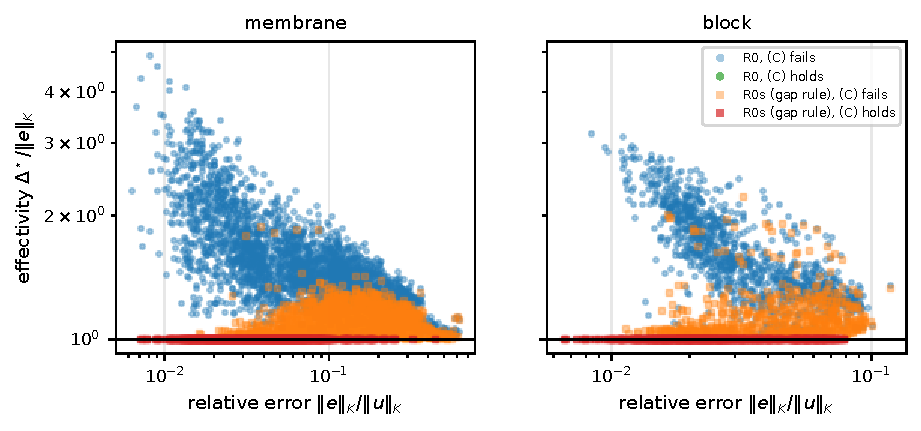
\includegraphics[width=\linewidth]{figures/fig_e1_effectivity}
\caption{E1. Effectivity against the relative energy error for R0 and R0s (gap rule). Points satisfying condition (C) lie on
$\mathrm{eff}=1$ (Corollary~\ref{cor:exact}); R0 does not satisfy (C) on the membrane. The figure illustrates the relation between condition (C) and the observed effectivity; it does not establish a convergence rate for approximations that violate (C).}
\label{fig:e1}
\end{figure}

\Cref{tab:e1} and \Cref{fig:e1} confirm that condition (C) yields unit effectivity to numerical precision. Its occurrence depends on the correction
method and benchmark. For the membrane, R0 never satisfies (C), whereas gap-based and multiplier-based snapping achieve $40\,\%$ and $35\,\%$,
respectively. For the block, the corresponding proportions are $8\,\%$, $45\,\%$, and $71\,\%$. When (C) is not satisfied, median effectivities
range from $1.01$ to $1.50$, with a maximum of $4.89$. All queries satisfy Theorem~\ref{thm:missed}, although the tightness of its bound and the
role of missed constraints in the largest effectivities remain unverified. Multiplier-based snapping achieves the highest exactness proportion on the
block but may reduce displacement accuracy through excessive snapping.

\subsection{E2: the support floor}\label{sec:e2}
Theorem~\ref{thm:support} establishes a positive asymptotic certificate floor when the multiplier support omits a strictly active constraint. This
is examined using predictions $\vu+\varepsilon\boldsymbol\varphi$, where $\boldsymbol\varphi=\mK^{-1}\mB\T\vlam$ is scaled so that
$\normK{\boldsymbol\varphi}=\normK{\vu}$, with $\varepsilon\in[10^{-6},10^{-1}]$. After correction on the exact strictly active set, each
approximation is certified using unrestricted S1 and two restricted supports: all rows except the largest-force active row $i^\ast$, and
$\Aplus\setminus\{i^\ast\}$. The floor $\sigma_S$ is computed offline using the exact multiplier. This controlled sequence tests the theoretical
result rather than representing typical reduced-order errors.

\begin{table}[t]
\centering\small
\caption{E2. At the smallest amplitude, the minimum over queries of the restricted certificate divided by the floor
$\sigma_S$ and by the full-S1 certificate; slope of the full-S1 certificate in the error (log--log). ``Violations'' counts
queries with ratio to $\sigma_S$ below $0.95$ or ratio to full S1 below $100$.}
\label{tab:e2}
\resizebox{\linewidth}{!}{% generated by experiments/tables.py; seeds [0, 1, 2]
\begin{tabular}{llrrrr}
\hline
problem & support $S$ & rate of full S1 & $\min\Delta^\star(\ell_S)/\sigma_S$ & $\min\Delta^\star(\ell_S)/\Delta^\star(\ell^\star)$ & violations \\
\hline
membrane & all rows but $i^\ast$ & 1.000 & 1.000 & 65044 & 0 \\
membrane & $\mathcal A_+\setminus\{i^\ast\}$ & 1.000 & 1.000 & 65044 & 0 \\
block & all rows but $i^\ast$ & 1.001 & 1.000 & 53449 & 0 \\
block & $\mathcal A_+\setminus\{i^\ast\}$ & 1.001 & 1.000 & 53449 & 0 \\
\hline
\end{tabular}
}
\end{table}

\begin{figure}[t]
\centering
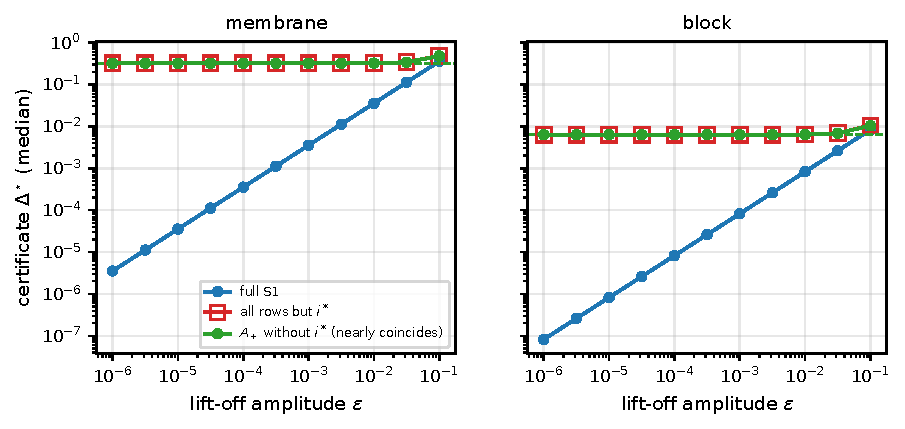
\includegraphics[width=\linewidth]{figures/fig_e2_support_floor}
\caption{E2. Median certificate against the amplitude $\varepsilon$ for full S1 and the two restricted supports (the two
restricted curves nearly coincide); dashed lines are the median floors $\sigma_S$, computed from the exact full-order multipliers for verification.}
\label{fig:e2}
\end{figure}

\Cref{tab:e2} and \Cref{fig:e2} show that unrestricted S1 converges linearly with the error, while both restricted certificates approach the predicted
floor. At the smallest amplitude, the restricted certificates exceed the unrestricted values by more than $5\times10^4$. The two supports produce
nearly identical certificate values, although their optimising multipliers differ (additional diagnostics are reported in
Appendix~\ref{app:e2diag}). This observed agreement is not asserted as a general identity. The result also holds for the block, whose correction
direction contains both positive and negative components and whose stiffness matrix is not an M-matrix.

\subsection{E3: property tests on random instances}\label{sec:e3}
The theoretical statements of Sections~\ref{sec:setting}--\ref{sec:failure} are tested on random constrained quadratic problems with full-row-rank
matrices $\mB$, symmetric positive-definite matrices $\mK$, and either $\mX=\mK$ or a random positive-definite $\mX$ with $s>1$. Four problem
sizes and five categories of feasible approximations are considered. Exact solutions are obtained from the condensed complementarity problem and
refined using equality-constrained KKT solves. Each of three seeds generates $1,000$ instances. No violations are observed under the specified
numerical tolerances (\Cref{tab:e3} in Appendix~\ref{app:e3}). The efficiency bound of Theorem~\ref{thm:efficiency} has a median ratio of
$0.87$ and a minimum of $0.34$, while Theorem~\ref{thm:missed} gives a median ratio of $0.71$. The lower bound of Theorem~\ref{thm:support}
is attained within $0.1\,\%$ in the most favourable instance. These tests verify algebraic consistency; contact-specific behaviour is examined
separately in E1 and E2.

\paragraph{Numerical verification adjustments.}
Four adjustments were made after the initial runs. First, the energy identity of Proposition~\ref{prop:gap} was evaluated in an algebraically
stable form to avoid cancellation, while direct energy differences were retained as diagnostics. Second, reference solutions were refined using
equality-constrained KKT solves. Third, rounding allowances proportional to $16\,n\,\varepsilon_{\rm mach}$ were introduced for the gap identity;
observed discrepancies remained within $2.4\,\%$ of these allowances. Finally, an unnecessary M-matrix check was removed from E2 because the
tested result does not require this property. All reported results use the revised verification procedures.

% Section 6: application. Corrections of reduced-order predictions as consistent / inconsistent feasible approximations.

\section{Application: corrections of reduced-order predictions}\label{sec:application}

The preceding analysis applies to any feasible displacement approximation. This section examines elementary corrections of Galerkin ROM predictions to illustrate the effects of active-set consistency on certificate efficiency and displacement accuracy. Let $\et:=\vu-\ut$ and $\gt:=\mB\ut-\vc$ denote the ROM displacement error and contact gap, respectively, and let $\pos{x}:=\max(x,0)$ componentwise.

\subsection{Right-inverse repair and snap-to-contact}

Define $\Bp:=\mB\T(\mB\mB\T)^{-1}$, so that $\mB\Bp=\mI$. The right inverse is evaluated using a thin QR factorisation of $\mB\T$, or directly when $\mB$ selects individual degrees of freedom. For a prescribed active set $\Ahat$, the corrected displacement is defined by
\begin{equation}\label{eq:snap}
  d_i:=\begin{cases}-\tilde g_i,& i\in\Ahat,\\ \pos{-\tilde g_i},& i\notin\Ahat,\end{cases}\qquad \uh:=\ut+\Bp\vd .
\end{equation}
For $\Ahat=\emptyset$, the correction reduces to the right-inverse feasibility repair R0, which eliminates penetration. For nonempty $\Ahat$, the snap-to-contact correction R0s additionally enforces zero gaps on the selected rows. Since $\mB\Bp=\mI$,
\begin{equation}\label{eq:snap-gap}
  \hat g_i=0\ \ (i\in\Ahat),\qquad \hat g_i=\pos{\tilde g_i}\ \ (i\notin\Ahat),
\end{equation}
ensuring feasibility for any $\Ahat$. Proposition~\ref{prop:certificate} therefore applies.

\subsection{Consistency and missed rows}

\begin{proposition}[Active-set consistency through snapping]\label{prop:snap}
If $\Aplus\subseteq\Ahat$, the correction \eqref{eq:snap} satisfies the bounded-effectivity estimate \eqref{eq:eff-consistent}.
\end{proposition}
\begin{proof}
By \eqref{eq:snap-gap}, $\hat g_i=0$ on $\Ahat\supseteq\Aplus$; apply Corollary~\ref{cor:effectivity}(b).
\end{proof}

When $\Ahat$ does not contain all strictly active constraints, the missed rows can be identified directly from the ROM prediction.

\begin{corollary}[missed rows of a snapped correction]\label{cor:snap-missed}
For \eqref{eq:snap}, $\Miss(\uh)=\{i\in\Aplus\setminus\Ahat:\tilde g_i>0\}$, and
\begin{equation}\label{eq:snap-missed}
  \vlam\T\gh=\sum_{i\in\Miss}\lambda_i\tilde g_i=-\vlam_{\Miss}\T\mB\et=-\vlam_{\Miss}\T\mB\ve\le m(\Miss)\min\big(\normK{\ve},\normK{\et}\big).
\end{equation}
\end{corollary}
\begin{proof}
By \eqref{eq:snap-gap}, $\hat g_i>0$ exactly for $i\notin\Ahat$ with $\tilde g_i>0$, and then $\hat g_i=\tilde g_i$. On $\Aplus$, $g_i=0$, so
$\tilde g_i=-(\mB\et)_i$ and $\hat g_i=-(\mB\ve)_i$. The bound is the Cauchy--Schwarz inequality, as in Theorem~\ref{thm:missed}.
\end{proof}

For R0, the missed rows correspond to strictly active constraints predicted as open by the ROM. Their contribution to the complementarity term is bounded by the ROM displacement error.

\subsection{The accuracy cost of snapping}

Although snapping can improve certificate efficiency, it may increase the displacement error by enforcing additional contact constraints.

\begin{proposition}[cost of snapping]\label{prop:snap-cost}
Let $\vp$ have entries $p_i=\pos{\tilde g_i}$ for $i\in\Ahat$ and $p_i=0$ otherwise, let $\uh_{R0}$ and $\uh_{s}$ be the corrections
\eqref{eq:snap} with $\emptyset$ and $\Ahat$, and $\beta:=\norm{\mK^{1/2}\Bp}_2$. Then
\begin{equation}\label{eq:snap-cost}
  \uh_{s}=\uh_{R0}-\Bp\vp,\qquad \big|\normK{\vu-\uh_s}-\normK{\vu-\uh_{R0}}\big|\le\normK{\Bp\vp}\le\beta\,\norm{\vp}_2 .
\end{equation}
Moreover, $p_i\le|(\mB\et)_i|$ for $i\in\Ahat\cap\Acon$ and $p_i\le g_i+|(\mB\et)_i|$ for $i\in\Ahat\setminus\Acon$.
\end{proposition}
\begin{proof}
The two corrections differ only on $\Ahat$, where $d_i^{s}-d_i^{R0}=-\tilde g_i-\pos{-\tilde g_i}=-\pos{\tilde g_i}$. The bound is the triangle
inequality. Finally $\tilde g=\vg-\mB\et$ with $g_i=0$ on $\Acon$.
\end{proof}

The correction cost depends on whether the snapped constraints belong to the exact contact set. Constraints in contact contribute at the order of the ROM error, whereas over-snapped constraints may introduce errors proportional to their nonzero exact gaps. Multiplier-based selection does not directly control this contribution, while gap-based selection provides an explicit bound.

\begin{corollary}[gap rule]\label{cor:gap-rule}
For $\Ahat_t:=\{i:\tilde g_i\le t\}$ with $t\ge0$:
\begin{enumerate}
\item[(a)] $\normK{\vu-\uh_s}\le\normK{\vu-\uh_{R0}}+\beta\,t\,|\Ahat_t|^{1/2}$, whatever the true contact set;
\item[(b)] $\Miss(\uh_s)\subseteq\{i\in\Aplus:|(\mB\et)_i|>t\}$; in particular, $\norm{\mB\et}_\infty\le t$ implies $\Aplus\subseteq\Ahat_t$ and
$\mathrm{eff}\le\frac2{\sqrt3}s$.
\end{enumerate}
\end{corollary}
\begin{proof}
(a) Every $p_i\le t$; apply Proposition~\ref{prop:snap-cost}. (b) A missed row has $\tilde g_i>t$, and $\tilde g_i=-(\mB\et)_i$ on $\Aplus$.
\end{proof}

The threshold $t$ balances active-set consistency against displacement accuracy. Increasing $t$ reduces the possibility of missed constraints but increases the upper bound on the correction error. The natural scale is $\norm{\mB\et}_\infty$, which is unavailable online; consequently, Section~\ref{sec:results} uses a fixed threshold. The constant $\beta$ depends on the mesh and, for a node-selection matrix $\mB$ with unit entries, satisfies $(\Bp)\T\mK\Bp=\mB\mK\mB\T$.


\section{Conclusions}\label{sec:conclusions}

This study investigates the efficiency and limitations of optimised-multiplier error certification for discrete frictionless contact problems. The derived efficiency bound identifies the complementarity between exact contact forces and approximate gaps as a key factor governing certificate sharpness. For the stiffness-based inner product, the surrogate-minimising multiplier is characterised as the solution of a contact problem with a shifted obstacle. This interpretation yields a necessary and sufficient condition for exact multiplier recovery and a sufficient condition for exact error certification. Two distinct limitations are established: contact inconsistency in the displacement approximation can cause worst-case square-root degradation, whereas excluding a strictly active constraint from the multiplier support produces a positive asymptotic certificate floor. Numerical experiments support all tested theoretical results and demonstrate that the occurrence of exact certification depends on the correction strategy. These findings highlight the importance of preserving contact consistency on strictly active constraints and ensuring adequate multiplier support in certified reduced-order contact models.

The conditions for exact certification and the efficiency bounds involve quantities from the unknown full-order solution, limiting their direct use in online assessment. Future work should therefore focus on developing computable indicators of contact consistency and certificate sharpness. Alternative estimators incorporating contact-set information may also overcome the square-root degradation established for the considered certificate family. Further investigations are needed to characterise intermediate convergence rates, assess parameter-dependent stiffness matrices and larger contact problems, and evaluate certification costs relative to full-order solutions. Incorporating discretisation error into the certification framework remains another important direction.


\appendix

\section{Random-instance verification table}\label{app:e3}

Table~\ref{tab:e3} summarises the verification of the theoretical results using random instances in experiment E3 (Section~\ref{sec:e3}). It reports the number of checks, violations, worst numerical margins, and ratios between the two sides of each inequality.

\begin{table}[H]
\centering\scriptsize
\caption{Verification of theoretical statements on $3000$ random instances (E3). Conditional statements are tested only when their assumptions hold. Lemma~\ref{lem:phi} is evaluated using S1 and two random nonnegative multipliers per instance, while Theorem~\ref{thm:support} is tested for two supports. The worst margin represents the minimum scaled inequality slack or the negative maximum scaled identity discrepancy; values above $-10^{-9}$ are accepted. The final column reports the median and range of the left-to-right bound ratio, with the lower-bound ratio defined in reverse order.}
\label{tab:e3}
\resizebox{\linewidth}{!}{% generated by experiments/tables.py; seeds [0, 1, 2]
\begin{tabular}{lrrrl}
\hline
statement & checks & violations & worst margin & lhs/rhs: median (min--max) \\
\hline
\cref{lem:phi}: $\Phi\le\Delta^2$ & 9000 & 0 & -2.2e-16 & 0.932 (0.750--1.000) \\
\cref{lem:phi}: $\Delta^2\le\frac43\Phi$ & 9000 & 0 & 6.1e-09 & 0.805 (0.750--1.000) \\
\cref{rem:inexact}: inexact S1 & 3000 & 0 & 4.5e-05 & 0.876 (0.412--1.000) \\
\cref{rem:inexact}: no factor $2/\sqrt3$ if $\eta(\ell^\star)=0$ & 1388 & 0 & -1.7e-13 & 1.000 (0.421--1.000) \\
\cref{thm:efficiency}: $\|e\|_K\le\Delta^\star$ & 3000 & 0 & -2.6e-13 & 0.717 (0.039--1.000) \\
\cref{thm:efficiency}: $\Delta^\star\le\frac{2}{\sqrt3}(s^2\|e\|^2+\lambda^T\hat g)^{1/2}$ & 3000 & 0 & 5.7e-05 & 0.866 (0.339--1.000) \\
\cref{thm:efficiency}: $\lambda^T\hat g\le m(\mathcal A_+)\|e\|$ & 3000 & 0 & 9.0e-04 & 0.000 (0.000--0.761) \\
\cref{cor:effectivity}: $\mathrm{eff}\le\frac{2}{\sqrt3}s$ if $\lambda^T\hat g=0$ & 1863 & 0 & 1.1e-01 & 0.866 (0.339--0.904) \\
\cref{thm:missed}: $\lambda^T\hat g=-\lambda_{\mathcal M}^TBe$ & 3000 & 0 & -5.7e-10 & identity \\
\cref{thm:missed}: $\lambda^T\hat g\le m(\mathcal M)\|e\|$ & 3000 & 0 & -5.7e-10 & 0.170 (0.000--0.847) \\
\cref{thm:missed}: effectivity bound & 3000 & 0 & 1.1e-01 & 0.708 (0.063--0.904) \\
\cref{cor:localized}: $\lambda^T\hat g\le\|\lambda_{\mathcal M}\|_2\|\hat g_{\mathcal M}\|_2$ & 915 & 0 & -1.7e-10 & 1.000 (0.048--1.000) \\
\cref{thm:support}: upper bound & 6000 & 0 & 5.7e-05 & 0.728 (0.272--1.000) \\
\cref{thm:support}: $(\sigma_S-\sqrt{\gamma_X}\|e\|)/\sqrt{\alpha_X}\le\Delta^\star$ & 6000 & 0 & 1.0e+00 & 0.842 (0.000--0.999) \\
\cref{thm:support}: $\sigma_S>0\iff\mathcal A_+\not\subseteq S$ & 6000 & 0 & -- & identity \\
\cref{prop:gap}: $J(\hat u)-J(u)=\frac12\|e\|^2+\lambda^T\hat g$ & 1837 & 0 & -5.8e-10 & identity \\
same, direct evaluation (diagnostic, rounding allowance) & 1837 & 0 & -1.9e-09 & identity \\
\cref{prop:gap}: $G=\frac12\bar\rho^2+\eta$ (up to rounding) & 1837 & 0 & -1.4e-09 & identity \\
\cref{prop:gap}: $\Delta^\star\le\sqrt{2G}$ & 1837 & 0 & -1.0e-10 & 1.000 (0.717--1.000) \\
\cref{prop:shifted}: S1 = shifted contact problem & 1837 & 0 & -1.0e-12 & identity \\
\cref{prop:shifted}: $\bar\rho=\|\hat u-u'\|_K$ & 1837 & 0 & -2.9e-13 & identity \\
\cref{prop:shifted}: feasibility & 1837 & 0 & 1.0e-09 & identity \\
\cref{cor:exact}: $\Delta^\star=\|e\|_K$ if $0\le\hat g\le2g$ & 1316 & 0 & -1.6e-10 & identity \\
\cref{cor:exact}: $\ell^\star=\lambda$ if $0\le\hat g\le2g$ & 1316 & 0 & -6.9e-14 & identity \\
\hline
\end{tabular}
}
\end{table}

\subsection{Supplementary numerical diagnostics}\label{app:e2diag}

In E2, the restricted certificates differ by at most $1\,\%$ for the membrane and $3\,\%$ for the block across all amplitudes, decreasing to $0.4\,\%$ for $\varepsilon\le10^{-3}$. Both supports have the same certificate floor because $\vlam$ vanishes outside $\Aplus$, although their certificate values are not generally identical. The larger support produces nonzero multiplier components outside $\Aplus$, reaching approximately $12\,\%$ and $40\,\%$ of the largest multiplier entry for the membrane and block, respectively. Differences on $\Aplus\setminus\{i^\ast\}$ reach approximately $3\,\%$ and $8\,\%$, respectively.

Initial verification of the energy identity in Proposition~\ref{prop:gap} produced discrepancies of $1.3\times10^{-9}$ and $2.6\times10^{-9}$ in two instances, exceeding the prescribed tolerance of $10^{-9}$. To reduce numerical cancellation, the identity was subsequently evaluated in the algebraically stable form
\[
J(\hat u)-J(u)=-\ve\T(\mK\vu-\vf)+\tfrac12\normK{\ve}^2.
\]
Reference solutions were also refined using equality-constrained KKT solves. Following the introduction of a rounding allowance for the gap identity, the observed discrepancies remained within $2.4\,\%$ of the allowance.


\bibliographystyle{unsrtnat}
\bibliography{refs}

\end{document}
